% Homework template for Algorithm Analysis and Design
% UPDATE: September 20, 2019 by Xu Rongchen
\documentclass[a4paper]{article}
\usepackage{ctex}
\ctexset{
proofname = \heiti{证明} %% set proof name
}
\usepackage{amsmath, amssymb, amsthm}
% amsmath: equation*, amssymb: mathbb, amsthm: proof
\usepackage{moreenum}
\usepackage{mathtools}
\usepackage{url}
\usepackage{bm}
\usepackage{enumitem}
\usepackage{graphicx}
\usepackage{subcaption}
\usepackage{booktabs} % toprule
\usepackage[mathcal]{eucal}

\usepackage{iidef} % set homework count
\usepackage{longtable}

% \usepackage[noend]{algpseudocode}
\usepackage{clrscode3e}

\thecoursename{算法分析与设计实验报告}
\theterm{2019年秋季学期}
\hwname{字符串匹配算法比较}
\slname{\heiti{解}}
\begin{document}
\courseheader
\theusername{徐荣琛}
\thestuno{2019214518}
\theinstitute{软件学院}

\info

\begin{enumerate}
  \setlength{\itemsep}{3\parskip}
  %% Homework Start here:
  %% \item to enumerate the problem ID: Format as 'HomeworkID.ProblemID'
  %% \begin{solution} XXXX \end{solution} is to make a solution
  %% \begin{proof} XXXX \end{proof} is to make a proof
  %% Suggest to use \input{path} command
  \textbf{1.实验要求}\\
  实现并测试Brute-Force、KMP、BM这三种字符串匹配算法并提交实验报告。字母表至少含有26个英文字母,
  0-9数字以及若干英文标点符号,要求有方便测试的图形界面,程序可输入txt文件做测试,能够处理含有一百万字符的
  txt文件。\\
  \bigskip

  \textbf{2.实验环境}\\
  此次实验代码采用Java语言实现,图形界面采用Java Swing实现,具体的实验环境及编译配置如下表所示:\\ \medskip
  \begin{tabular}{c|c}
    \hline\hline
    处理器 & Intel(R) Core(TM) i7-8850H CPU @ 2.60GHz \\ \hline
    内存 & 16GB\\ \hline
    操作系统& Mac OS X 10.14.6\\ \hline
    Java版本& Java(TM) SE Runtime Environment (build 1.8.0)\\ \hline
    \hline\hline
  \end{tabular}\\
  \bigskip

  \textbf{3.实验内容}\\
  \textbf{3.1 有关算法的实现}\\
  \medskip
  3.1.1 Brute-Force:\\
  对于Text串的每个位置,暴力Pattern串向后进行匹配,如果发现失配则进入下一个Text串的位置,直至
  字符串访问结束。最坏情况下的时间复杂度$O(mn)$。\\
  \medskip
  3.1.2 KMP:\\
  预处理前缀函数$\pi$(时间复杂度为$O(m)$),然后遍历对于Text串的每个位置,使用Pattern串进行匹配,
  如果发现失配,则利用前缀函数的性质直接继续匹配Text串当前位置以及Pattern当前位置的前缀函数位置继续
  匹配,直至Text访问结束。总体的时间复杂度为$O(m+n)$。\\
  \medskip
  3.1.3 BM:\\
  预处理前缀函数$bmBc$(坏字符)和$bmGs$(好偏移,利用最大重叠后缀计算)两个数组(时间复杂度为$O(m)$)。
  对于Text串的每个位置$i$,从$i+m$处向前匹配Pattern串,如果失配,则$i$右移$bmBc$和$bmGs$得到的
  可行偏移量的较大值。不断匹配直至Text访问结束。总体的时间复杂度为$O(m+n)$。\\
  \medskip
  \textbf{3.2 实现优化}\\
  (1)$bmBc$中,对于字符串的每一位字符(1字节),使用256上限整数取代,避免建立字典的数据结构。\\
  (2)对于多次访问的数组,从ArrayList转化为int[]或char[]类型,提高随机访问效率。
  
  \medskip

  \medskip
  \textbf{3.3 不同规模下的求解实验}\\
  \medskip
  3.3.1 实验概要:\\
  在Text串长度$10^6$,$10^7$,$10^8$三个数据规模,Patten串长度$5$,$10$,$50$,$100$情况下进行对比实验。
  实验用例随机生成,实验结果进行相互的对比测试。\\
  \medskip
  3.3.2 实验结果:\\
  相互的对比测试未发现错误,表明了三种算法实现的正确性。具体实验时间如下所示。单位ms。
  % \resizebox{\linewidth}{!}{ 
    \begin{center}
      \begin{tabular}{c|cccccc}\hline\hline
        规模(T,P)      &Brute Force  &KMP        &BM       \\\hline
        $10^6,5$      &7.91         &9.02       &7.08   \\
        $10^6,10$     &6.81         &7.70       &4.64   \\
        $10^6,50$     &7.09         &7.81       &1.43   \\
        $10^6,100$    &6.94         &7.55       &1.09  \\
        $10^7,5$      &28.33        &23.77      &19.89     \\
        $10^7,10$     &32.99        &35.83      &17.17   \\
        $10^7,50$     &30.74        &24.75      &8.68   \\
        $10^7,100$    &33.80        &28.49      &6.84   \\
        $10^8,5$      &232.25       &191.29     &111.23   \\
        $10^8,10$     &212.29       &186.65     &69.44   \\
        $10^8,50$     &249.48       &219.27     &37.46   \\
        $10^8,100$    &228.57       &198.66     &45.29   \\
        \hline\hline
      \end{tabular}
    \end{center}

  % }\\

  \medskip

  3.3.3 实验分析:\\
  分析上述数据,可以得到一些结论:

  (1)Brute Force方法的实际时间消耗和KMP相近,而BM展现出来最好且非常明显的速度优势。\\
  (2)随着Test串的长度的增大,三种算法的时间消耗均相应增加。\\
  (3)Brute Force方法和KMP算法受Pattern串长度的影响不大。而对于BM算法,可以发现在绝大多数情况下,随着
  Pattern串长度增加,匹配时间反而减小。这与算法实际相符,因为Pattern串越长,实际BM算法可能跳动的距离也随之
  增大,于是算法可能更快结束。

  \textbf{3.4 图形界面展示}\\
  实现的GUI界面如下图所示。(可直接允许项目文件中的GUI.jar得到)
  \begin{center}
    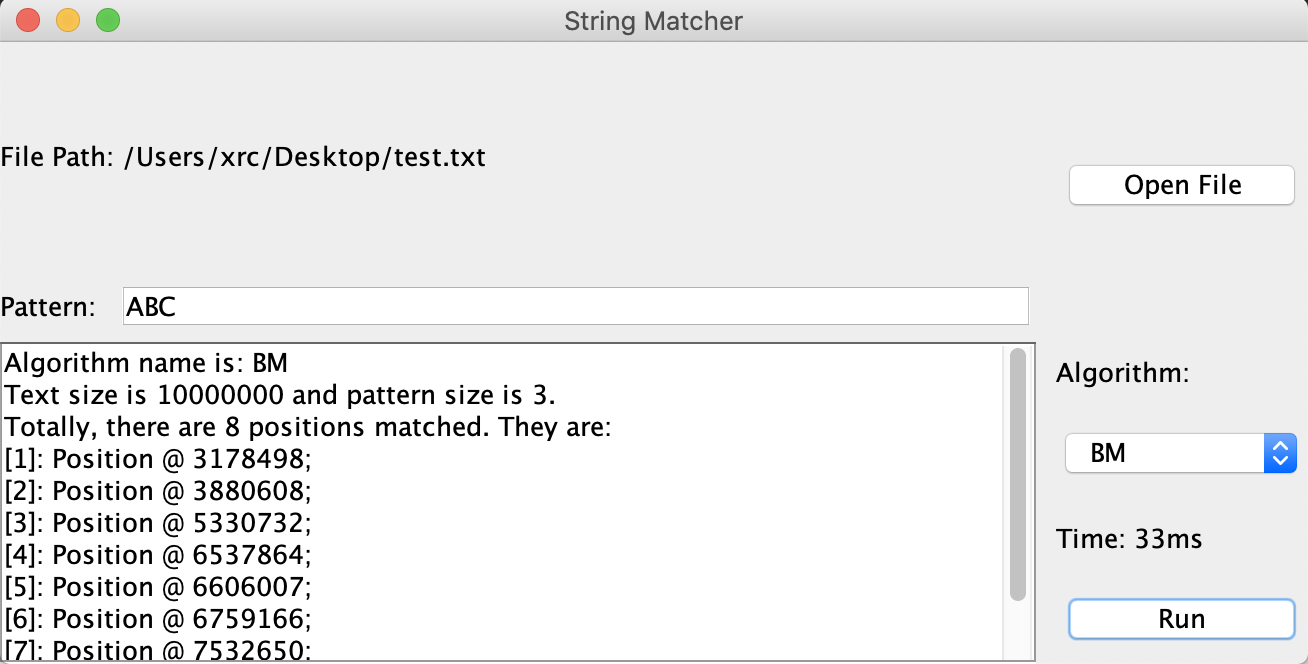
\includegraphics[scale=0.4]{Pictures/gui.png}
  \end{center}
\end{enumerate}


\end{document}